\subsection{型付けの例}

\begin{frame}
  \frametitle{型が付く例/付かない例}
  コード生成器
  \begin{align*}
    e & = \red{\cResetz} ~~\cforin{i = 0}{n} \\
      & \phantom{=}~~~~\blue{\cResetz} ~~\cforin{j = 0}{m} \\
      & \phantom{=}~~~~~~ \blue{\cShiftz}~\blue{k_2}~\to~ \red{\cShiftz}~\red{k_1}~\to~ \magenta{\cLet~y=\green{t}~\cIn} \\
      & \phantom{=}~~~~~~~~ \red{k_1}~(\blue{k_2}~(a\cArrays{i}{j} = b\cArray{i} + y))
  \end{align*}

  \pause
  生成されるコード
  \begin{columns}
    \begin{column}{0.5\textwidth}%% [横幅] 0.2\textwidth = ページ幅の 20 %
      \center
      
\includegraphics[clip,height=1cm]{./img/batsu.png}
      \begin{align*}
        e & \too \magenta{\Let ~y ~= ~\green{a[i][j]} ~\In} \\
          & \phantom{\too}~~~~ \forin{i = 0}{n} \\
          & \phantom{\too}~~~~~~\forin{j = 0}{m} \\
          & \phantom{\too}~~~~~~~~a[i][j] = b[i] + y \\
      \end{align*}
    \end{column}

    \begin{column}{0.5\textwidth}%% [横幅] 0.2\textwidth = ページ幅の 20 %
      \center
      
\includegraphics[height=1cm]{./img/maru.png}
      \begin{align*}
        e & \too \magenta{\Let ~y ~= ~\green{7} ~\In} \\
          & \phantom{\too}~~~~ \forin{i = 0}{n} \\
          & \phantom{\too}~~~~~~\forin{j = 0}{m} \\
          & \phantom{\too}~~~~~~~~a[i][j] = b[i] + y \\
      \end{align*}
    \end{column}
  \end{columns}
\end{frame}

\begin{frame}
  \center
  \huge{安全なコードにのみ型をつけるにはどうすればよいか}
\end{frame}

\subsection{型システム}

\begin{frame}
  \frametitle{環境識別子 EC によるスコープ表現 [Taha+2003] [Sudo+2014]}
  \begin{center}
    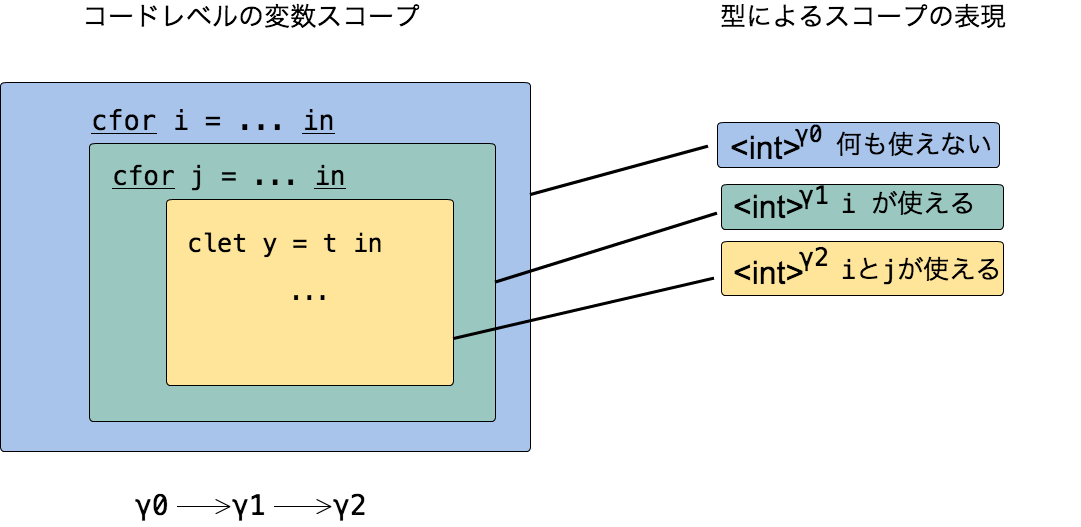
\includegraphics[clip,height=5.7cm]{./img/ec.png}
  \end{center}
  \begin{flushright}
    $\gamma_i ... \text{Refined Environment Classifier}$
  \end{flushright}
\end{frame}

\begin{frame}
  \frametitle{ECの洗練化 (本研究)}
  \begin{onlyenv}<1>
    \flushleft
    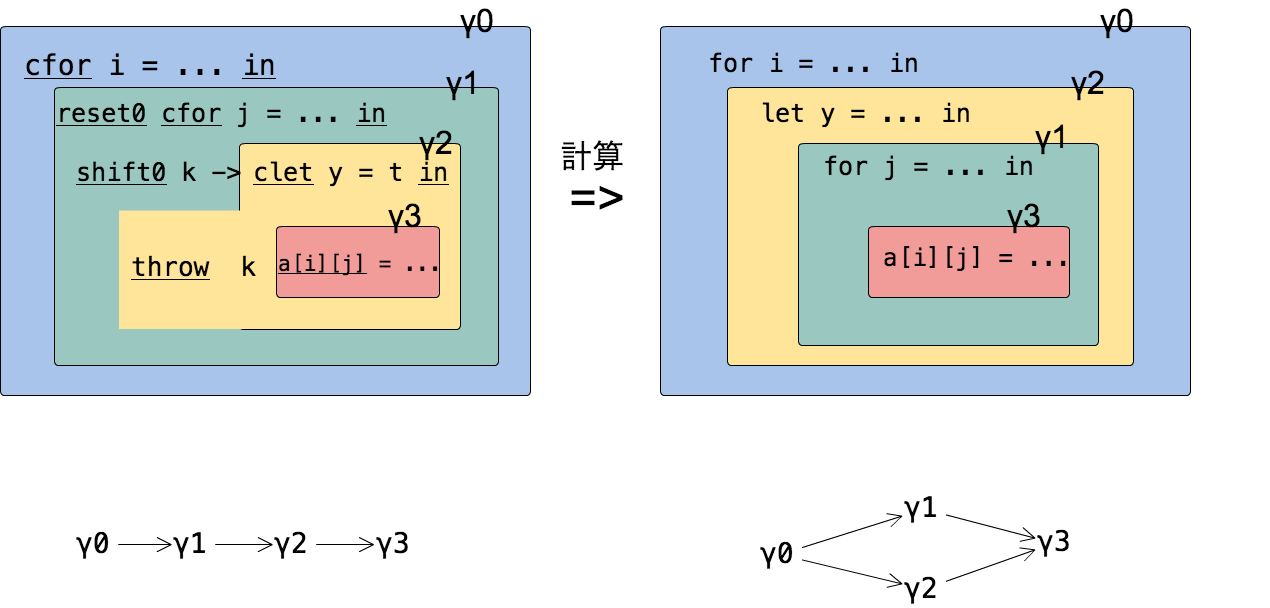
\includegraphics[clip,height=6cm]{./img/ecex1.png}
  \end{onlyenv}

  \begin{onlyenv}<2>
    \flushleft
    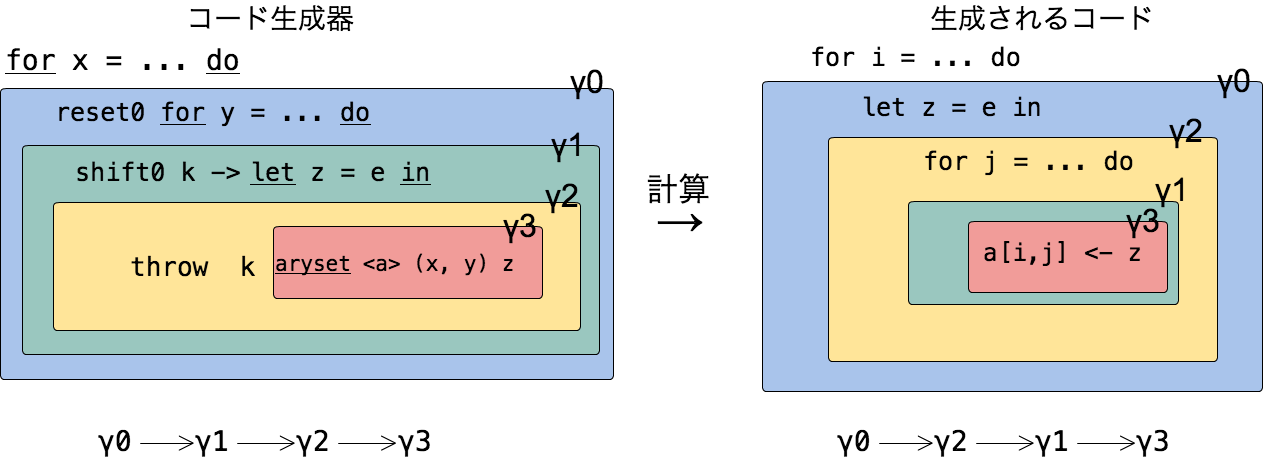
\includegraphics[clip,height=6cm]{./img/ecex.png}
  \end{onlyenv}
\end{frame}

\begin{frame}
  \frametitle{ECのジョイン}
  \flushleft
  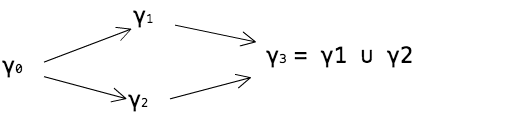
\includegraphics[clip,height=3cm]{./img/ecgraph.png}
  \begin{itemize}
  \item<2-> $\gamma_1$ のコードレベル変数は $\gamma_2$ では使えない
  \item<3-> $\gamma_2$ のコードレベル変数は $\gamma_1$ では使えない
  \item<4-> $\gamma_1, \gamma_2$ のコードレベル変数は $\gamma_3$ で使える
  \item<5->[$\Rightarrow$] Sudoらの体系に $\cup$ を追加
  \end{itemize}
\end{frame}

\begin{frame}[fragile]
  \frametitle{コード生成+shift0/reset0 の型システム (の一部)}
  Typing rule for code-level let (derived rule):
  \[
    \infer[(\gamma_1~\text{is eigen var})]
    {\Gamma \vdash \clet{x}{e_1}{e_2} ~:~ \codeT{t_2}{\gamma}}
    {\Gamma \vdash e_1 ~:~ \codeT{t_1}{\gamma}
      &\Gamma,~\gamma_1 \ord \gamma,~x:\codeT{t_1}{\gamma_1} \vdash
      e_2 ~:~ \codeT{t_2}{\gamma_1}
    }
  \]

  Typing rule for code-level reset0:
  \[
    \infer{\Gamma \vdash \cresetz{e} ~:~ \codeT{t}{\gamma}}
    {\Gamma \vdash e ~:~ \codeT{t}{\gamma}}
  \]

  Typing rule for code-level shift0:
  \[
    \infer{\Gamma \vdash \cshiftz{k}{e} ~:~ \codeT{t_1}{\gamma_1}}
    {\Gamma,~k:\contT{\codeT{t_1}{\gamma_1}}{\codeT{t_0}{\gamma_0}}
      \vdash e ~:~ \codeT{t_0}{\gamma_0}
      & \Gamma \models \gamma_1 \ord \gamma_0
    }
  \]

  Typing rule for code-level throw:
  \[
    \infer[(\gamma_3~\text{is eigen var})]
    {\Gamma,~k:\contT{\codeT{t_1}{\gamma_1}}{\codeT{t_0}{\gamma_0}}
      \vdash \cthrow{k}{e} ~:~ \codeT{t_0}{\gamma_2}}
    {\Gamma,~
      \red{\gamma_3 \ord \gamma_1,~
      \gamma_3 \ord \gamma_2}
      \vdash e ~:~ \codeT{t_1}{\gamma_3}
      & \Gamma \models \gamma_2 \ord \gamma_0
    }
  \]

\end{frame}

\section{まとめと今後の課題}

\begin{frame}
  \frametitle{まとめと今後の課題}
  まとめ
  \begin{itemize}
    % \item コードの言語にshift0 reset0 を組み込んだ言語の設計を行った
  \item コード生成言語の型システムに shift0/reset0 を組み込んだ 型システムの設計を完成させた.
  \item 安全なコードの場合に型が付くこと,安全でないコードの場合には型が付かないように意図通りに型システムが設計できていることをみた
  \end{itemize}

  % \vspace{1in}
  \vspace{\baselineskip}

  今後の課題
  \begin{itemize}
    % \item answer type modification に対応した型システムを設計し,(subject reduction 等の)健全性の証明を行う
  \item 設計した型システムの健全性の証明(Subject recudtion等)を行い,実装を完成させる
  \end{itemize}
\end{frame}

%%% Local Variables:
%%% mode: japanese-latex
%%% TeX-master: "slide"
%%% End:
